\chapter{Prototype Alpha: Experience} 

Experience prototyping engages the designers, clients and users with the prototypes. This helps the designer understand, explore or communicate what it is like to engage with the product. According to Buchenau and Suri 2000, Experience Prototyping is particularly powerful in three activities within prototyping, see list below.

\vspace{0.5cm}
\begin{enumerate}
    \item Understanding existing user experiences and context
    \item Exploring and evaluating design ideas
    \item Communicating ideas to an audience
\end{enumerate}
\vspace{0.5cm}

Experience Prototyping is essentially a cheap and effective way to assess various parts of design or technical solution during the product development.\cite{christer}

\section{Minimum Viable Product}
The success of Pre-Alpha proved the functionality of the concept. To follow an experience prototyping course, the company needs a product that can provide feedback from customers. Therefor, the Alpha will be designed as a Minimum Viable Product (MVP), one of the most important lean start-up techniques. A MVP is a product with just enough features to satisfy early customers, and to provide feedback for future product development. Developers can deploy this product to a potential user as an early adopter. Giving a user a functional product with less features gives more power to the user to give feedback on what is missing. If a company is in a constant reworking prototyping stage, this strategy lowers the cost, maximizes the information and avoids building products that customers do not want. The final, complete set of features is only designed and developed after considering feedback from the product's initial users.
\cite{MVP}
\par
Alpha was completed as an MVP in February 2017. It is designed to extend the functionality requirements from Pre-Alpha and satisfy other customer features such as comfort, lightweight, handling and braking. A remodelled sit-ski is mounted onto a rig that has improved mountain board trucks with brakes attached at each end, see figure \ref{alpha}. 

\vspace{0.5cm}
\begin{figure}[htb!]
    \centering
    {\setlength{\fboxsep}{0pt}\setlength{\fboxrule}{1pt}
    \fbox{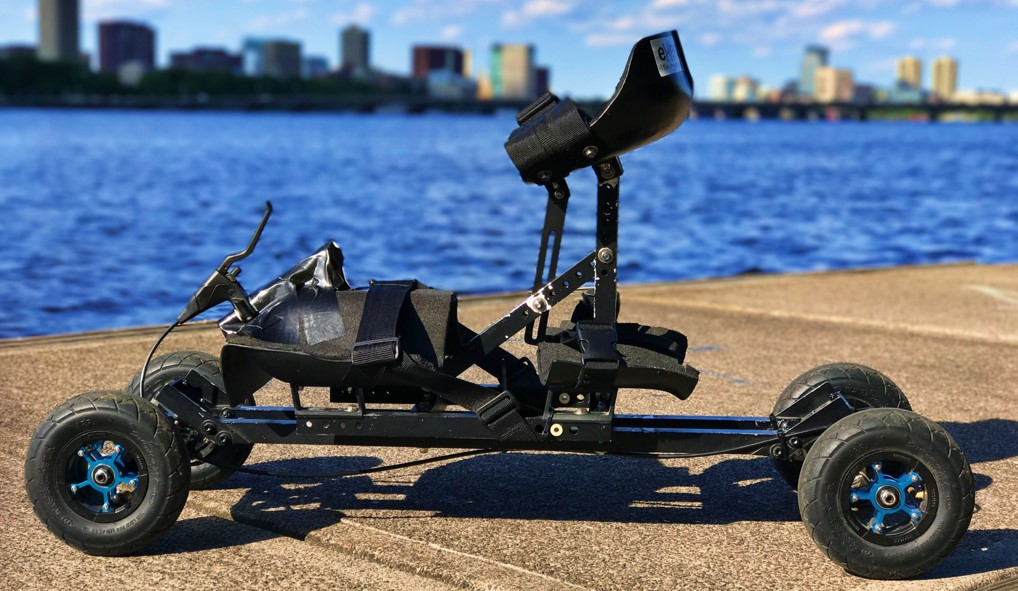
\includegraphics[height=0.50\textwidth]{figures/exero/spike.jpg}}}
    \captionsetup{justification=centering}
    \caption{Prototype Alpha}
    \floatfoot{\textit{Source: Exerotech Database} \cite{exerotechdatabase}}
    \label{alpha}
\end{figure}
\vspace{0.5cm}

Alpha's sit-ski seat can be radially adjusted. The knee and calf supports can be individually adjusted vertically on the sit-ski and the sit-ski itself can be moved vertically on the rig. The sit-ski and rig are made up of 25x25x2.5mm 6061 T6 aluminum profiles. The seat, knee and calf supports are made by casting plastic and are layered with closed-cell foams for cushioning. All supports have belt straps to hold the body in place. All adjustments are done through un-screwing M6 screws and bolts on the sit-ski and rig and re-screwing them in new positions.
\par
A 6mm thick aluminum plate is welded at an angle of 35{\degree} at each end of the rig. Here, Trampa Vertigo Trucks are attached with M4 screws and bolts. The trucks have one spring and damper on each side of a rotational center. These springs can be individually adjusted allowing for the possibility of moving the users weight symmetry. The Innova Slick Cut 8-inch tires are set up with hydraulic brakes on each of the two front wheels. The manual braking lever is mounted in the middle of the knee support, see figure \ref{alpha}.

PICTURE of weight symmetry and trucks

%table with weight and other stats!
\section{Testing and User Feedback}
\setlength\floatsep{0pt}
\setlength\intextsep{0pt}
\begin{wrapfigure}[11]{r}{0.40\textwidth}
    \begin{center}
    {\setlength{\fboxsep}{0pt}\setlength{\fboxrule}{0.5pt}
    \fbox{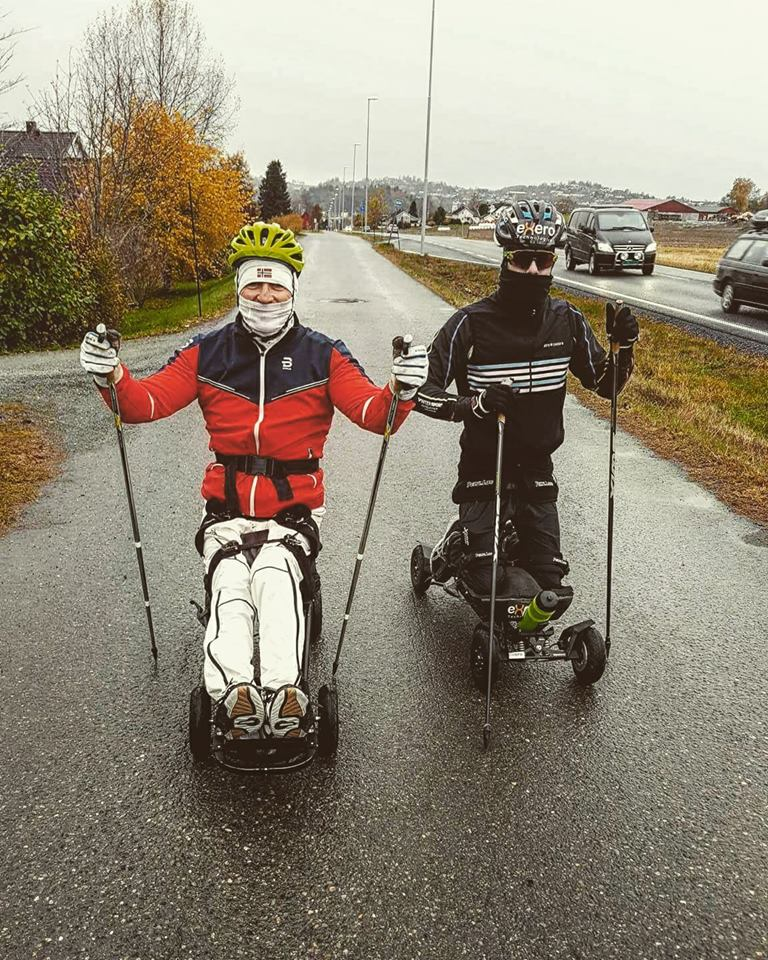
\includegraphics[width=0.4\textwidth]{figures/exero/spiketest.jpg}}}
    \caption{Espen Aksnes testing Alpha}
    \floatfoot{\textit{Source: Exerotech Database} \cite{exerotech}}
    \label{alphatest}    
    \end{center}
\end{wrapfigure}

Alpha was meant as a prototype to provide feedback for future product development. Throughout the spring and summer of 2017 Alpha was tested with over 30 different users with different paraplegia, see figure \ref{alphatest}. Assessment reports from every user were documented to give an overview and feedback of the user experience, see Appendix \ref{appendix:user_feedback}.
WRITE MORE

\section{Discussion}

